\documentclass[tikz]{standalone}
\usepackage{tikz}
\usetikzlibrary{decorations.pathreplacing}
\usepackage{setspace}
\usepackage[UTF8]{ctex}
\usetikzlibrary{fit}
\usetikzlibrary{backgrounds} 
\begin{document}
	\begin{spacing}{0.7}
		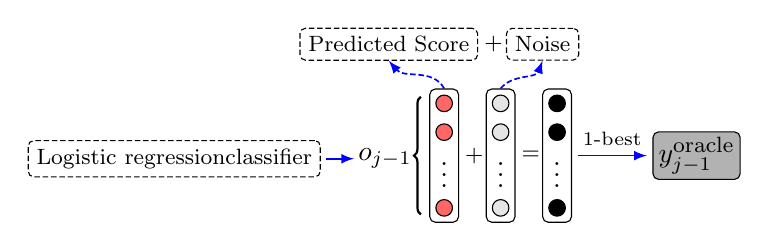
\begin{tikzpicture}
			\tikzstyle{annotation} = [draw,inner sep=3pt,rounded corners=2pt,font=\footnotesize,align=center,dash pattern=on 2pt off 1pt]
			\tikzstyle{point} = [draw,circle,inner sep=0pt,minimum size=6pt]
			
			\node [annotation] (logit) at (0,0){\textrm{Logistic regression \\ classifier};
			\node [anchor=west] (o) at ([xshift=1em]logit.east){$o_{j-1}$};
			
			\node[anchor=west,point,fill=red!60] (p11) at ([xshift=0.5em,yshift=2em]o.east){};
			\node[anchor=north,point,fill=red!60] (p12) at ([yshift=-0.4em]p11.south){};
			\node[anchor=north,inner sep=0pt] (d1) at ([yshift=-0.15em]p12.south){$\vdots$};
			\node[anchor=north,point,fill=red!60] (p13) at ([yshift=-0.4em]d1.south){};
			
			\node[anchor=west,point,fill=gray!20] (p21) at ([xshift=1.4em]p11.east){};
			\node[anchor=north,point,fill=gray!20] (p22) at ([yshift=-0.4em]p21.south){};
			\node[anchor=north,inner sep=0pt] (d2) at ([yshift=-0.15em]p22.south){$\vdots$};
			\node[anchor=north,point,fill=gray!20] (p23) at ([yshift=-0.4em]d2.south){};
			
			\node[anchor=west,point,fill=black] (p31) at ([xshift=1.4em]p21.east){};
			\node[anchor=north,point,fill=black] (p32) at ([yshift=-0.4em]p31.south){};
			\node[anchor=north,inner sep=0pt] (d3) at ([yshift=-0.15em]p32.south){$\vdots$};
			\node[anchor=north,point,fill=black] (p33) at ([yshift=-0.4em]d3.south){};
			
			%background
    		\begin{pgfonlayer}{background}
        		\node [draw,rectangle,inner sep=2pt,rounded corners=2pt] [fit = (p11)(p12) (p13)] (box0) {};
        		\node [draw,rectangle,inner sep=2pt,rounded corners=2pt] [fit = (p21)(p22) (p23)] (box1) {};
        		\node [draw,rectangle,inner sep=2pt,rounded corners=2pt] [fit = (p31)(p32) (p33)] (box2) {};
    		\end{pgfonlayer}
			
			\node[anchor=west,inner sep=0pt] at ([xshift=0.2em]box0.east){\footnotesize +};
			\node[anchor=west,inner sep=0pt] at ([xshift=0.2em]box1.east){\footnotesize =};
			\node[draw,fill=gray!60,rounded corners=2pt,inner sep=2pt, align=center] (oracle) at ([xshift=4.5em]box2.east){$y_{j-1}^{\textrm{\footnotesize oracle}}$};
			\node [anchor=south,annotation] (ps) at ([xshift=-2em,yshift=1em]box0.north){\textrm{Predicted Score}};
			\node [anchor=west,annotation] (noise) at ([xshift=1em]ps.east){\textrm{Noise}};
			\node[anchor=west,inner sep=0pt] at ([xshift=0.2em]ps.east){\footnotesize +};
			
			\draw[-latex,line width=0.6pt,color=blue] ([xshift=0.2em]logit.east) -- ([xshift=0.2em]o.west);
			\draw[decorate,decoration={brace,mirror},line width=0.8pt] ([xshift=-0.3em,yshift=-0.3em]box0.north west) -- ([xshift=-0.3em,yshift=0.3em]box0.south west);
			\draw[-latex,line width=0.6pt,color=blue] ([xshift=0.2em]box2.east) -- node[above,color=black]{\scriptsize 1-best} ([xshift=-0.2em]oracle.west);
			\draw[-latex,dash pattern=on 2pt off 1pt,line width=0.6pt,out=120,in=-50,color=blue] (box0.north) to (ps.south);
			\draw[-latex,dash pattern=on 2pt off 1pt,line width=0.6pt,out=50,in=-110,color=blue] (box1.north) to (noise.south);
		\end{tikzpicture}
	\end{spacing}
\end{document} 